\section{Progress}
\label{sec:progress}
\subsection{Weeks 1-2}
During the first 2 weeks of term time was spent on the Specificationa as well as attempting to establish a strong
base to the project in which I can build on for the rest of the project.

\begin{figure}
    \centering
    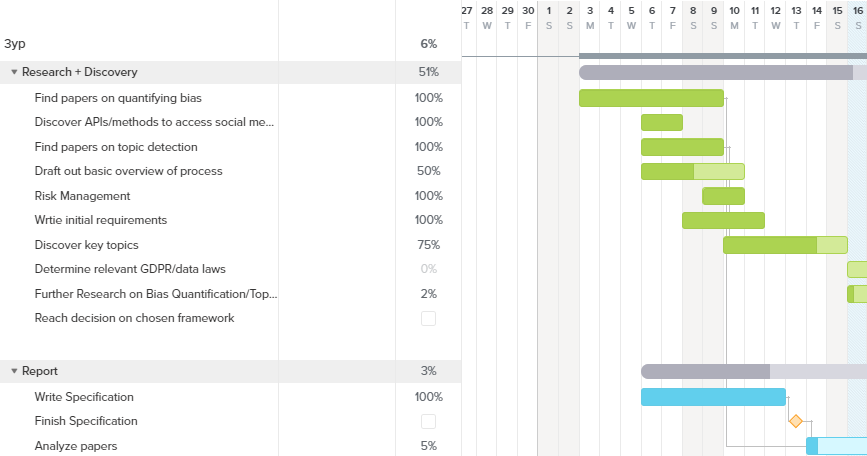
\includegraphics[width=0.5\textwidth]{../images/timetableweek1-2.png}
    \caption{Timetable for weeks 1-2}
    \label{fig:timetableweek1-2}
\end{figure}

As seen from this figure I met most of the deadlines set for the first 2 weeks of the project. I did miss some deadlines
Including: Drafting an overview of the process; Discovering key topics; and starting looking into GDPR and Data Protection laws.
Although it would have been beneficial to have achieved the latter 2 in the list above, the first objective was probably infeasible
for the first 2 weeks of the project - as further research is required to determine where I want this project taking.\\\\

I also completed a few extra tasks slightly early this week. I established an API connection to Twitter as well as reading up on
API access to Facebook and Instagram. As mentioned in my specification, I am going to stick with using Twitter as a base for
this project but may look into using Facebook and Instagram as well.\\\\

Finally I started looking more into the papers I laid out in the spec. Specifically looking into Pythia and how they overcome
the challenge of twitter posts usually being short and not containing much information.